% Options for packages loaded elsewhere
\PassOptionsToPackage{unicode}{hyperref}
\PassOptionsToPackage{hyphens}{url}
%
\documentclass[
  12pt,
]{article}
\usepackage{lmodern}
\usepackage{amssymb,amsmath}
\usepackage{ifxetex,ifluatex}
\ifnum 0\ifxetex 1\fi\ifluatex 1\fi=0 % if pdftex
  \usepackage[T1]{fontenc}
  \usepackage[utf8]{inputenc}
  \usepackage{textcomp} % provide euro and other symbols
\else % if luatex or xetex
  \usepackage{unicode-math}
  \defaultfontfeatures{Scale=MatchLowercase}
  \defaultfontfeatures[\rmfamily]{Ligatures=TeX,Scale=1}
  \setmainfont[]{Times New Roman}
\fi
% Use upquote if available, for straight quotes in verbatim environments
\IfFileExists{upquote.sty}{\usepackage{upquote}}{}
\IfFileExists{microtype.sty}{% use microtype if available
  \usepackage[]{microtype}
  \UseMicrotypeSet[protrusion]{basicmath} % disable protrusion for tt fonts
}{}
\makeatletter
\@ifundefined{KOMAClassName}{% if non-KOMA class
  \IfFileExists{parskip.sty}{%
    \usepackage{parskip}
  }{% else
    \setlength{\parindent}{0pt}
    \setlength{\parskip}{6pt plus 2pt minus 1pt}}
}{% if KOMA class
  \KOMAoptions{parskip=half}}
\makeatother
\usepackage{xcolor}
\IfFileExists{xurl.sty}{\usepackage{xurl}}{} % add URL line breaks if available
\IfFileExists{bookmark.sty}{\usepackage{bookmark}}{\usepackage{hyperref}}
\hypersetup{
  pdftitle={Is big tech greenwashing?},
  pdfauthor={Amanda Booth and Ricky Prophete},
  hidelinks,
  pdfcreator={LaTeX via pandoc}}
\urlstyle{same} % disable monospaced font for URLs
\usepackage[margin=2.54cm]{geometry}
\usepackage{longtable,booktabs}
% Correct order of tables after \paragraph or \subparagraph
\usepackage{etoolbox}
\makeatletter
\patchcmd\longtable{\par}{\if@noskipsec\mbox{}\fi\par}{}{}
\makeatother
% Allow footnotes in longtable head/foot
\IfFileExists{footnotehyper.sty}{\usepackage{footnotehyper}}{\usepackage{footnote}}
\makesavenoteenv{longtable}
\usepackage{graphicx,grffile}
\makeatletter
\def\maxwidth{\ifdim\Gin@nat@width>\linewidth\linewidth\else\Gin@nat@width\fi}
\def\maxheight{\ifdim\Gin@nat@height>\textheight\textheight\else\Gin@nat@height\fi}
\makeatother
% Scale images if necessary, so that they will not overflow the page
% margins by default, and it is still possible to overwrite the defaults
% using explicit options in \includegraphics[width, height, ...]{}
\setkeys{Gin}{width=\maxwidth,height=\maxheight,keepaspectratio}
% Set default figure placement to htbp
\makeatletter
\def\fps@figure{htbp}
\makeatother
\setlength{\emergencystretch}{3em} % prevent overfull lines
\providecommand{\tightlist}{%
  \setlength{\itemsep}{0pt}\setlength{\parskip}{0pt}}
\setcounter{secnumdepth}{5}

\title{Is big tech greenwashing?}
\usepackage{etoolbox}
\makeatletter
\providecommand{\subtitle}[1]{% add subtitle to \maketitle
  \apptocmd{\@title}{\par {\large #1 \par}}{}{}
}
\makeatother
\subtitle{\url{https://github.com/amandafbooth/BoothProphete_ENV872_EDA_FinalProject}}
\author{Amanda Booth and Ricky Prophete}
\date{}

\begin{document}
\maketitle

\newpage
\tableofcontents 
\listoftables 
\listoffigures 
\newpage

\hypertarget{rationale-and-research-questions}{%
\section{Rationale and Research
Questions}\label{rationale-and-research-questions}}

As the world searches for climate change mitigation strategies in the
face of apocalyptic climate projections and escalating real-world
effects, the need to decarbonize the global economy has placed
increasing societal and political pressure on companies to limit their
emissions. Part of this pressure has come from the Environmental,
Social, and Governance investing movement, which focuses on
sustainability as a key part of identifying material risks and growth
opportunities for companies.

Corporations have responded to the decarbonization challenge posed by
these external forces by self-disclosing their carbon footprints along
with action plans for reducing them over a specified time horizon.
However, there are 2 key issues with the self-disclosure model:

\begin{itemize}
\item
  Current emissions accounting and reporting practices have not been
  harmonized, leading to differential approaches to carbon accounting.
\item
  Given a lack of oversight in emissions reporting and the nature of
  informational asymmetries between organizations and investors,
  companies face perverse incentives to understate their carbon
  footprint and/or otherwise mischaracterize their progress toward
  decarbonization.
\end{itemize}

There have been recent efforts to address these issues. In March of
2022, the Securities and Exchange Commission (SEC) proposed rule
amendments that would require companies to incorporate specific
climate-related information in their statements and reports. This rule
would also impose additional disclosure requirements on organizations
that have made public commitments to take steps to address climate
change. As part of their rationale for the proposed rule changes, the
SEC noted both the need to harmonize disclosure standards and a desire
to mitigate attempts by companies to engage in ``green-washing'' or
``climate-washing''.

It is in this context that we sought to understand the extent to which
companies might be engaged in green- or climate-washing, and whether
organizations engaged in these behaviors possessed specific attributes
that could reliably predict the propensity of such behavior. To
investigate this, we reviewed a partial dataset from the Carbon
Disclosure Project (CDP), which is a nonprofit that manages a global
carbon emissions disclosure system. As CDP data is paywalled, we were
able to access this partial dataset via a study published in
\emph{Nature Communications} (\emph{Nature}) (Klaaßen \& Stoll). This
dataset and its attributes are described in greater detail in our
Dataset Information section.

Our primary research question was the following:

\begin{itemize}
\tightlist
\item
  What attributes are the strongest predictors for emissions reporting
  discrepancies?
\end{itemize}

Over the course of our work, our dataset inspired an additional
question:

\begin{itemize}
\tightlist
\item
  What attributes are the strongest predictors for an organization's
  total energy consumption?
\end{itemize}

\newpage

\hypertarget{dataset-information}{%
\section{Dataset Information}\label{dataset-information}}

\hypertarget{data-retrieval}{%
\subsection{Data Retrieval}\label{data-retrieval}}

For this analysis, we used data analyzed in a \emph{Nature} study that
took data from 2019 CDP reports. CDP, a carbon footprint registry for
companies and municipalities, conducts an in-depth questionnaire that
inquires about the details of what entities do and don't include in
their carbon emissions reporting. The \emph{Nature} study compared what
technology companies published in their official company reports to what
companies reported in CDP questionnaires and found technology companies
often under reported emissions in official company reports. The data
from nature came in the form of an Excel Workbook with many panels. We
converted three panels into CSVs for analysis in R:

\begin{itemize}
\tightlist
\item
  Company information
\item
  Emissions predictors
\item
  Reporting inconsistencies
\end{itemize}

Table 1: Data Information

\begin{longtable}[]{@{}ll@{}}
\toprule
\begin{minipage}[b]{0.58\columnwidth}\raggedright
\textbf{Detail}\strut
\end{minipage} & \begin{minipage}[b]{0.36\columnwidth}\raggedright
\textbf{Description}\strut
\end{minipage}\tabularnewline
\midrule
\endhead
\begin{minipage}[t]{0.58\columnwidth}\raggedright
Data Source\strut
\end{minipage} & \begin{minipage}[t]{0.36\columnwidth}\raggedright
Nature Communications\strut
\end{minipage}\tabularnewline
\begin{minipage}[t]{0.58\columnwidth}\raggedright
Retrieved from\strut
\end{minipage} & \begin{minipage}[t]{0.36\columnwidth}\raggedright
\url{https://www.nature.com/articles/s41467-021-26349-x}\strut
\end{minipage}\tabularnewline
\begin{minipage}[t]{0.58\columnwidth}\raggedright
Variables Used\strut
\end{minipage} & \begin{minipage}[t]{0.36\columnwidth}\raggedright
Company, Sales, Profits, Assets, Market value, Company report, CDP
emissions, Emission reports deviation, Reporting inconsistency ratio,
Total energy consumption\strut
\end{minipage}\tabularnewline
\begin{minipage}[t]{0.58\columnwidth}\raggedright
Data Collection Year\strut
\end{minipage} & \begin{minipage}[t]{0.36\columnwidth}\raggedright
2019\strut
\end{minipage}\tabularnewline
\bottomrule
\end{longtable}

\hypertarget{data-wrangling}{%
\subsection{Data Wrangling}\label{data-wrangling}}

We processed our data by selecting relevant columns in each panel. These
are described below:

\hypertarget{company-information}{%
\subsubsection{Company Information}\label{company-information}}

For this panel, we began by identifying and slicing relevant rows of
information pertaining to corporations of interest. We then selected
columns with relevant attributes, and renamed them like so: Company,
Industry, Country, Sales, Profits, Assets, Market Value, CDP Score 2019.
Next, we converted column values to numeric data by removing special
characters and changing the variable class.

\hypertarget{emissions-predictors}{%
\subsubsection{Emissions Predictors}\label{emissions-predictors}}

For this panel, we began by isolating values of interest. We sliced
relevant rows, then selected columns with relevant attributes Next, we
transposed the data so that each row contained consumption data for a
specific company. We renamed the resulting columns Company and Total
energy consumption. Finally, we removed special characters and converted
column values to numeric data.

\hypertarget{reporting-inconsistencies}{%
\subsubsection{Reporting
Inconsistencies}\label{reporting-inconsistencies}}

For this panel, we again selected and filtered a specific variable of
interest, in this case the difference between publicly reported
emissions and emissions reported to CDP. We then transposed the data and
renamed columns Company, Company.report, CDP, and Deviation. We
substituted ``na''s for missing data, then removed special characters
and converted existing data to numeric. Finally, we created a new
column, populated by variables, derived from dividing the Deviation
value by the CDP value. We named this column Inconsistency Ratio.

Once our individual datasets were processed, we combined them into a
single dataframe. To accomplish this, we created a new dataframe named
company\_profiles by left joining the Company Information dataset with
the Reporting Inconsistencies datset. We then left joined the Emissions
Predictors dataset to this new company\_profiles dataframe. To assist
our analysis, we concluded by filtering out ratios equal to 1 by
dropping ``na''s.

\newpage

\hypertarget{exploratory-analysis}{%
\section{Exploratory Analysis}\label{exploratory-analysis}}

We reviewed our dataset and identified the top offenders by
inconsistency ratio. The top 5 are shown here:

\begin{longtable}[]{@{}ll@{}}
\caption{Top 5 Companies by Highest Reporting Inconsistency
Ratio}\tabularnewline
\toprule
Company & Inconsistency\_ratio\tabularnewline
\midrule
\endfirsthead
\toprule
Company & Inconsistency\_ratio\tabularnewline
\midrule
\endhead
Samsung SDI & 0.9994994\tabularnewline
SAP & 0.9620065\tabularnewline
Adobe & 0.9005902\tabularnewline
Salesforce.com & 0.8326687\tabularnewline
IBM & 0.7553958\tabularnewline
\bottomrule
\end{longtable}

We also reviewed the extent to which our variables of interest might be
correlated. These results are published here:

\begin{figure}
\centering
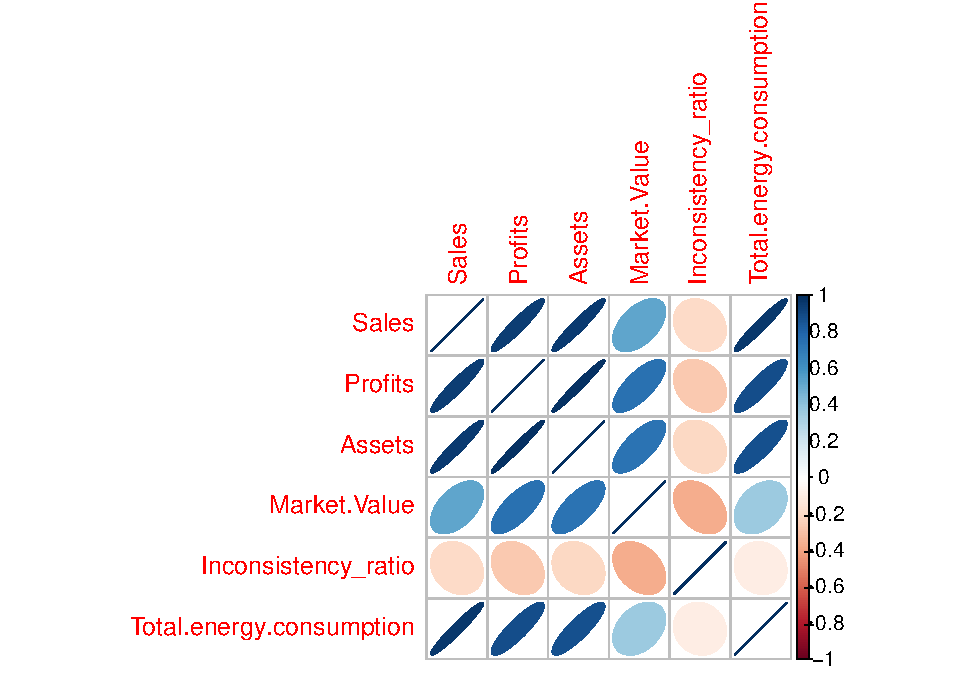
\includegraphics{BoothProphete_Report_files/figure-latex/correlations-1.pdf}
\caption{Correlation matrix of interested variables}
\end{figure}

\newpage

\hypertarget{analysis}{%
\section{Analysis}\label{analysis}}

\hypertarget{question-1-what-attributes-are-the-strongest-predictors-for-emissions-reporting-discrepancies}{%
\subsection{Question 1: What attributes are the strongest predictors for
emissions reporting
discrepancies?}\label{question-1-what-attributes-are-the-strongest-predictors-for-emissions-reporting-discrepancies}}

To answer this question, we leveraged a linear model:

\begin{figure}
\centering
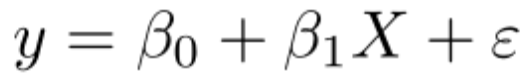
\includegraphics{./BoothProphete_Report_files/figure-latex/Linear_regression.png}
\caption{A Simple Linear Regression}
\end{figure}

Our outcome of interest was the Inconsistency Ratio derived as part of
our wrangling process. Our explanatory variables were Sales, Profits,
Assets, and Market Value. These were regressed against our outcome
variable. We did not find any statistically significant relationship
between these variables and the outcome of interest.

\begin{verbatim}
## 
## Call:
## lm(formula = Inconsistency_ratio ~ Market.Value, data = company_profiles2)
## 
## Residuals:
##      Min       1Q   Median       3Q      Max 
## -0.60852 -0.22922  0.09443  0.30961  0.40890 
## 
## Coefficients:
##                Estimate Std. Error t value Pr(>|t|)   
## (Intercept)   6.155e-01  1.421e-01   4.331   0.0019 **
## Market.Value -4.626e-07  4.622e-07  -1.001   0.3430   
## ---
## Signif. codes:  0 '***' 0.001 '**' 0.01 '*' 0.05 '.' 0.1 ' ' 1
## 
## Residual standard error: 0.3934 on 9 degrees of freedom
##   (17 observations deleted due to missingness)
## Multiple R-squared:  0.1002, Adjusted R-squared:  0.0001967 
## F-statistic: 1.002 on 1 and 9 DF,  p-value: 0.343
\end{verbatim}

\hypertarget{question-2-what-attributes-are-the-strongest-predictors-for-an-organizations-total-energy-consumption}{%
\subsection{Question 2: What attributes are the strongest predictors for
an organization's total energy
consumption?}\label{question-2-what-attributes-are-the-strongest-predictors-for-an-organizations-total-energy-consumption}}

To answer this question, we leveraged the same methodology described in
our first question, with the only change occuring to our outcome of
interest. This new outcome of interest was total energy consumption
(MWh). Assets turned out to be the attribute that could predict total
energy consumption with the highest degree of statistical confidence.
This statistic is shown here:

\begin{verbatim}
## 
## Call:
## lm(formula = Total.energy.consumption ~ Assets, data = company_profiles2)
## 
## Residuals:
##       Min        1Q    Median        3Q       Max 
## -11037692   -705586   -413200    782164  15038161 
## 
## Coefficients:
##              Estimate Std. Error t value Pr(>|t|)    
## (Intercept) 2.676e+05  9.282e+05   0.288    0.776    
## Assets      3.566e+01  7.633e+00   4.672 8.72e-05 ***
## ---
## Signif. codes:  0 '***' 0.001 '**' 0.01 '*' 0.05 '.' 0.1 ' ' 1
## 
## Residual standard error: 3921000 on 25 degrees of freedom
##   (1 observation deleted due to missingness)
## Multiple R-squared:  0.4661, Adjusted R-squared:  0.4448 
## F-statistic: 21.83 on 1 and 25 DF,  p-value: 8.723e-05
\end{verbatim}

\begin{verbatim}
## 
## Call:
## lm(formula = Total.energy.consumption ~ Market.Value, data = company_profiles2)
## 
## Residuals:
##      Min       1Q   Median       3Q      Max 
## -6432376 -1604207 -1029920    79948 22428849 
## 
## Coefficients:
##               Estimate Std. Error t value Pr(>|t|)  
## (Intercept)  1.638e+06  1.068e+06   1.533   0.1378  
## Market.Value 7.646e+00  3.360e+00   2.276   0.0317 *
## ---
## Signif. codes:  0 '***' 0.001 '**' 0.01 '*' 0.05 '.' 0.1 ' ' 1
## 
## Residual standard error: 4884000 on 25 degrees of freedom
##   (1 observation deleted due to missingness)
## Multiple R-squared:  0.1716, Adjusted R-squared:  0.1385 
## F-statistic: 5.179 on 1 and 25 DF,  p-value: 0.03169
\end{verbatim}

\begin{verbatim}
## 
## Call:
## lm(formula = Total.energy.consumption ~ Sales, data = company_profiles2)
## 
## Residuals:
##       Min        1Q    Median        3Q       Max 
## -11795715   -669847   -235930    791088  13979353 
## 
## Coefficients:
##              Estimate Std. Error t value Pr(>|t|)    
## (Intercept) 152725.25  949887.65   0.161   0.8736    
## Sales           54.25      11.75   4.618   0.0001 ***
## ---
## Signif. codes:  0 '***' 0.001 '**' 0.01 '*' 0.05 '.' 0.1 ' ' 1
## 
## Residual standard error: 3942000 on 25 degrees of freedom
##   (1 observation deleted due to missingness)
## Multiple R-squared:  0.4604, Adjusted R-squared:  0.4388 
## F-statistic: 21.33 on 1 and 25 DF,  p-value: 0.0001002
\end{verbatim}

\begin{verbatim}
## 
## Call:
## lm(formula = Total.energy.consumption ~ Profits, data = company_profiles2)
## 
## Residuals:
##       Min        1Q    Median        3Q       Max 
## -11679157  -1152251   -510779    641968  16210298 
## 
## Coefficients:
##              Estimate Std. Error t value Pr(>|t|)    
## (Intercept) 1.150e+06  9.006e+05   1.277 0.213352    
## Profits     2.203e+02  5.455e+01   4.038 0.000449 ***
## ---
## Signif. codes:  0 '***' 0.001 '**' 0.01 '*' 0.05 '.' 0.1 ' ' 1
## 
## Residual standard error: 4174000 on 25 degrees of freedom
##   (1 observation deleted due to missingness)
## Multiple R-squared:  0.3947, Adjusted R-squared:  0.3705 
## F-statistic:  16.3 on 1 and 25 DF,  p-value: 0.0004495
\end{verbatim}

\newpage

\hypertarget{summary-and-conclusions}{%
\section{Summary and Conclusions}\label{summary-and-conclusions}}

We did not find a statistically significant relationship between
companies' reporting discrepancy ratios and variables that indicate
size. As expected, we found a relationship between total energy
consumption and size indicators. But surprisingly the indicator with the
most confidence was value of assets.

\begin{figure}
\centering
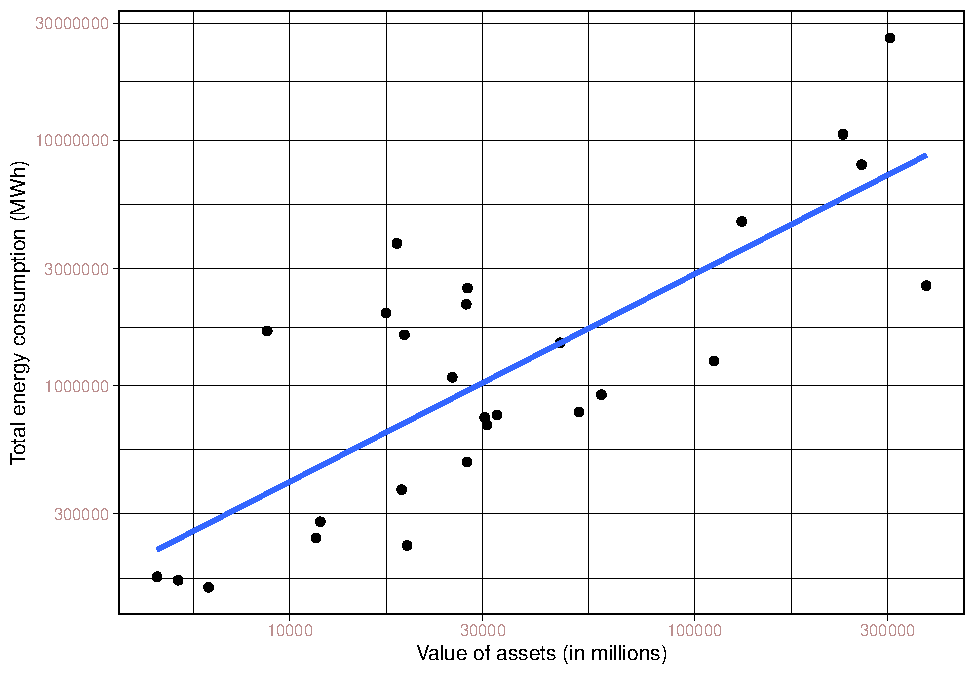
\includegraphics{BoothProphete_Report_files/figure-latex/plot1-1.pdf}
\caption{Relationship between asset value and total energy consumption}
\end{figure}

Our assumption that ``big tech'' would show more reporting discrepancies
was not borne out in the data we analyzed. In future analyses on this
topic, we would ideally have access to more CDP reports and more
corporate reports in order to have a sample size that allows for more
statistically accuracy.

\newpage

\hypertarget{references}{%
\section{References}\label{references}}

Klaaßen, Lena and Stoll, Christian. ``Harmonizing Corporate Carbon
Footprints.'' Nature News, Nature Publishing Group, 22 Oct.~2021,
\url{https://www.nature.com/articles/s41467-021-26349-x}.

\end{document}
